%----------------------------------------------------------------------------
\chapter{Jegyzőkönyv}
%----------------------------------------------------------------------------

%----------------------------------------------------------------------------
\section{Első feladat}
%----------------------------------------------------------------------------
A ’6.mat’ fájl betöltése után a kapott adatokat megfeleztük, egyik felét tanítás céljából, másik felét tesztelés céljából használtuk fel.

\lstinputlisting[style=Matlab-editor]{figures/m05/matlab-1.m}\label{Matlab1}

A \figref{poi}~ábrán látható a kapott eredmény.

\begin{figure}[!h]
	\centering
	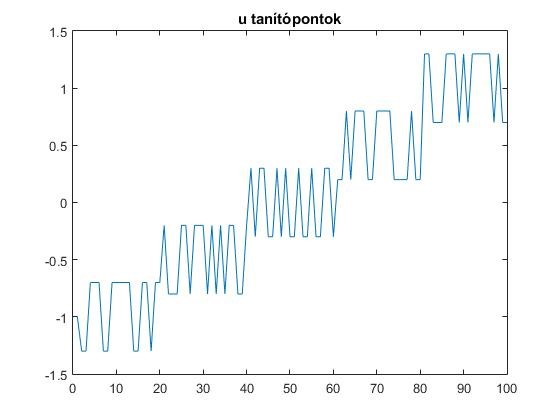
\includegraphics[width=69mm, keepaspectratio]{figures/m05/u_1.jpg}\hspace{5mm}
	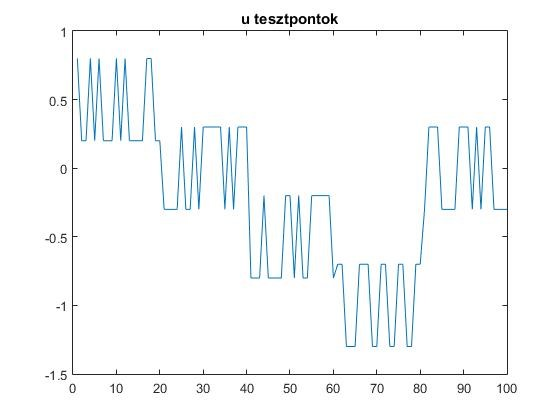
\includegraphics[width=69mm, keepaspectratio]{figures/m05/u_2.jpg}\\\vspace{5mm}
	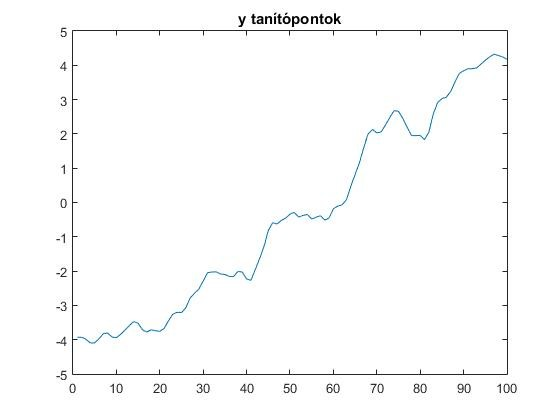
\includegraphics[width=69mm, keepaspectratio]{figures/m05/y_1.jpg}\hspace{5mm}
	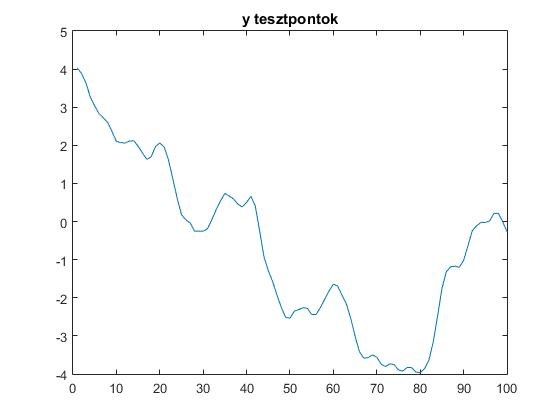
\includegraphics[width=69mm, keepaspectratio]{figures/m05/y_2.jpg}
	\caption{Tanító és tesztpontok}
	\label{fig:poi}
\end{figure}
\newpage

%----------------------------------------------------------------------------
\section{Második feladat}
%----------------------------------------------------------------------------
A rendszer inicializálásához a matlab egy beépített függvényét, a ’genfis2()-t használtuk fel. A függvény szubsztarktív klaszterezéssel állítja elő a szabálybázist. A működéséhez a tanítópontokat, a rájuk adott választ, és a klasztersugarat kellett megadnunk.
\lstinputlisting[style=Matlab-editor]{figures/m05/matlab-2.m}
A klasztersugár csökkentésével, a szabálybázist alkotó összefüggések száma növekszik. 



%----------------------------------------------------------------------------
\section{Harmadik feladat}
%----------------------------------------------------------------------------
\lstinputlisting[style=Matlab-editor]{figures/m05/matlab-3.m}

\begin{figure}[!h]
	\centering
	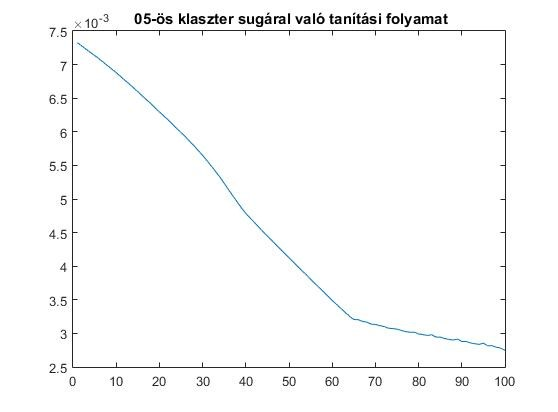
\includegraphics[width=90mm, keepaspectratio]{figures/m05/3.jpg}
\end{figure}


%----------------------------------------------------------------------------
\section{Negyedik feladat}
%----------------------------------------------------------------------------

Az ANFIS rendszer tesztelése következett ebben a feladatban. A tesztelés során a kapott Simulink modellt használtuk fel. A teszt eredményei a következő ábrákon láthatóak:

\begin{figure}[!h]
	\centering
	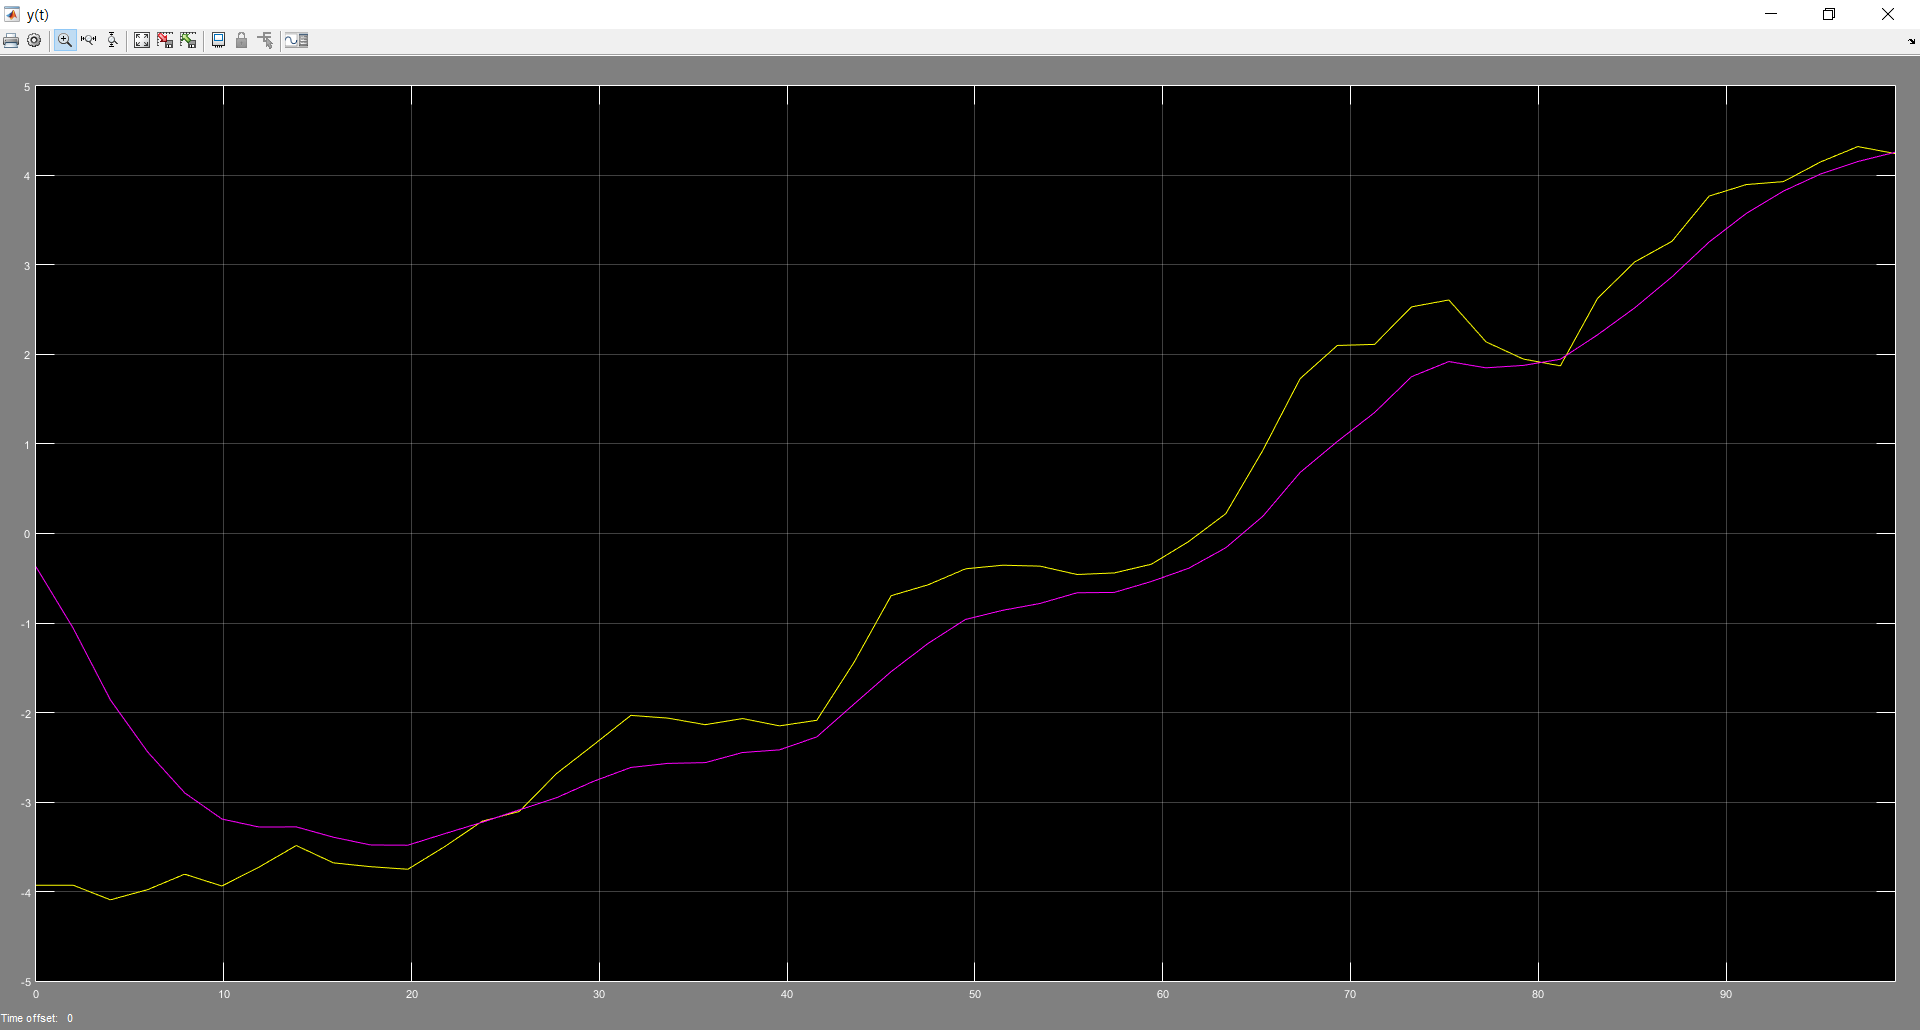
\includegraphics[width=150mm, keepaspectratio]{figures/m05/4_1.png}
	\caption{Az ANFIS rendszer kimenete és a mért érték}
\end{figure}
\begin{figure}[!h]
	\centering
	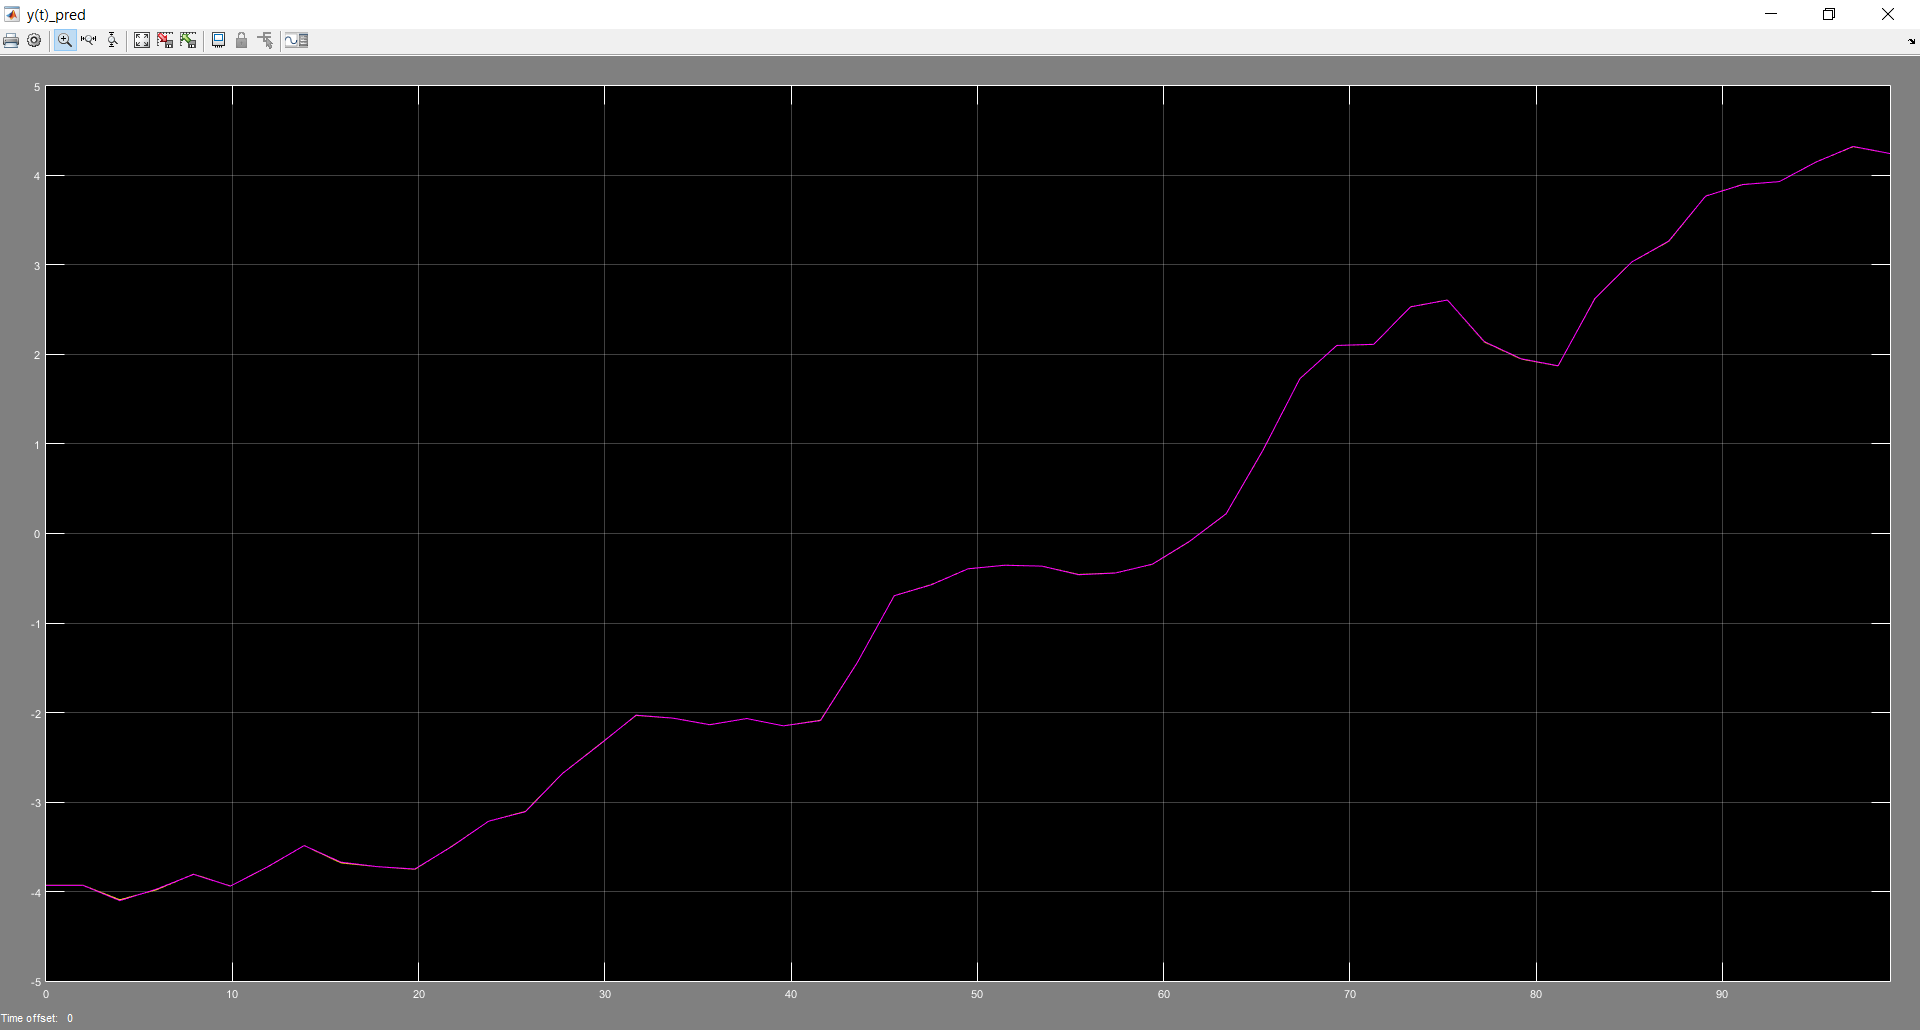
\includegraphics[trim=0mm 0mm 0mm 10mm, clip, width=150mm, keepaspectratio]{figures/m05/4_2.png}
	\caption{A prediktált kimenet és a mért kimenet}
\end{figure}
\begin{figure}[!h]
	\centering
	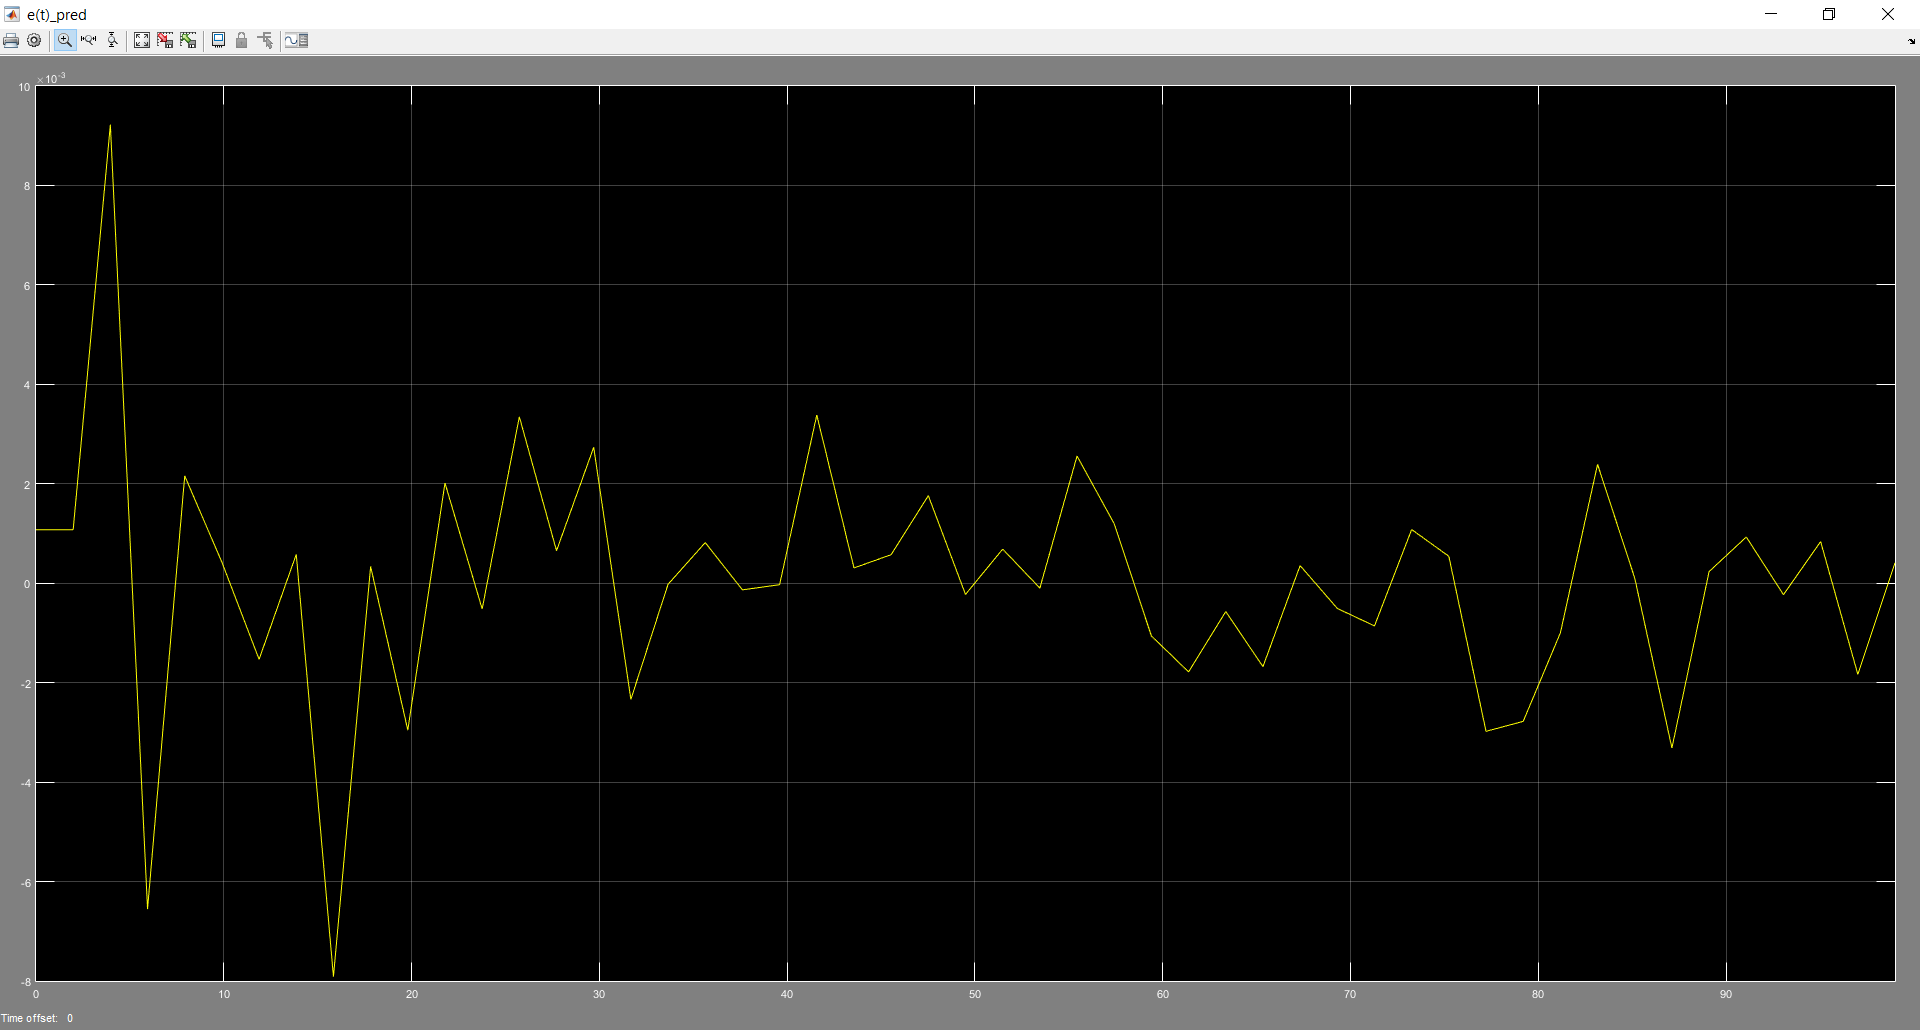
\includegraphics[trim=0mm 0mm 0mm 10mm, clip, width=150mm, keepaspectratio]{figures/m05/4_3.png}
	\caption{A prediktált kimenet és a mért kimenet közti eltérés}
\end{figure}

\newpage
%----------------------------------------------------------------------------
\section{Ötödik feladat}
%----------------------------------------------------------------------------
Az initANFIS függvény:
\lstinputlisting[style=Matlab-editor]{figures/m05/matlab-5.m}


%----------------------------------------------------------------------------
\section{Összegzés}
%----------------------------------------------------------------------------
A feladatok megoldása közben kipróbáltuk, hogy milyen eredményre jutunk amennyiben dinamikus viselkedést alkalmazunk. Dinamikus viselkedés esetén a rendszer bemenete nem más, mint az igazi, valós rendszer bemenete, kimenetére viszont a az ANFIS rendszer kimenetét használjuk. 
A predikció esetében a valós rendszert szimuláljuk, és a szimulált rendszer bemeneti és kimeneti értékeit használjuk fel az ANFIS-nál. A mérés során kiderült, hogy a predikció ad pontosabb eredményt.























